\subsection{Temporal Policy Switching: an identical-prompt falsification test}

TPDR measures response shape, not decision quality. As a stronger behavioral test, we introduce the \emph{Temporal Policy Switching (TPS)} benchmark, in which the visible prompt is held byte-identical and only the hidden $\Tau$ scalar varies. Each item asks an agent to choose exactly one of four labelled actions (REUSE, REFRESH, ASK, SUMMARIZE). Six policy families with different freshness thresholds (cache reuse, session continuation, API freshness, safety advice, calendar planning, market data) prevent a single global rule from solving the benchmark. Templates 8--11 of each family form a held-out prompt split; the entire \texttt{market\_data} family is fully held out for compositional generalization. Items are evaluated at nine $\Tau$ values from $10\,\mathrm{s}$ to $7\,\mathrm{d}$. The principal test is the \emph{hidden-only} condition: no time text appears in the prompt, so any above-vanilla accuracy must come from the hidden channel. The \emph{prompt\_only} condition writes the time directly into the prompt (with the chrono channel zeroed) and serves as the prompt-text baseline.

We pre-specified three hypotheses. \textbf{H1}: under hidden-only prompts, \CI{} raises policy accuracy above vanilla. \textbf{H2}: refresh probability rises monotonically with $\log\Tau$ under \CI{} on hidden-only items. \textbf{H3}: under prompt/\CI{} conflict, \CI{} alters the channel-follow rate. All three hypotheses are \emph{falsifiable}: if they fail, the behavioral claim narrows accordingly.

\textbf{Baselines and ceilings.} The benchmark is solvable from $(\Tau, \text{family})$ alone: a logistic regression on $\chi(\Tau)$ plus a family one-hot achieves 1.000 on held-in templates and 1.000 on held-out templates, but drops to 0.556 on the held-out \texttt{market\_data} family. A $\chi(\Tau)$-only classifier (no family) achieves 0.622, confirming that family identity carries most of the discriminative signal. The rule-oracle row reports the conceptual effective-$\Tau$ label function; the implemented \texttt{tau\_ci}-only oracle in the artifact has hidden-only accuracy 1.000 and overall accuracy 0.829 because prompt-only items intentionally have no hidden scalar. These anchors are ceilings, not learned baselines.

\textbf{Result (H1: hidden-only).} \emph{H1 fails for \CI{} v15s and is only weakly supported by the chrono-only ablation.} Vanilla Qwen 2.5 3B reaches 0.349 on hidden-only items. \CI{} v15s seed~0 reaches 0.340 (\emph{below} vanilla); across three seeds the hidden-only cross-seed mean is $0.344\pm0.005$, indistinguishable from vanilla. The chrono-only ablation (chrono trained, LoRA frozen at zero) reaches 0.387, a modest $+0.039$ over vanilla. This pattern suggests that the LoRA surface trained alongside the chrono channel during v15 training does not help, and may interfere, when the task is policy selection without any visible time string.

\textbf{Result (H2: monotonicity).} \emph{H2 fails: refresh probability does not rise with $\log\Tau$ under \CI{} v15s.} The Pearson correlation between $\log\Tau$ and $P(\text{REFRESH})$ on hidden-only items is $r=-0.184$ for seed 0, $r=-0.329$ for seed 1, $r=-0.299$ for seed 2 (cross-seed mean $r=-0.270$), all negative. Vanilla is essentially flat ($r=-0.000$), confirming the absence of a time signal. The negative slope under \CI{} indicates the chrono channel as trained on CLOCK + SILENT-GAP + PHASE does not transfer to a cache/session/freshness policy axis without task-specific supervision.

\textbf{Result (H3: conflict, inconclusive).} The original conflict generation contained 108 \emph{fake conflict} items (in the \texttt{market\_data} family the threshold of $10\,\mathrm{s}$ equals the short-side prompt $\Tau$, so $\text{gold}_{\text{scalar}}{=}\text{gold}_{\text{prompt}}$). We exclude these from the conflict tables. The corrected conflict rates (Table~\ref{tab:tps-conflict}; $n=540$ real conflicts per adapter) show vanilla following the visible prompt at 0.530 (the only signal it has) and \CI{} v15s seed~0 following the hidden scalar at 0.394 versus following the prompt at 0.496. Cross-seed scalar-follow under \CI{} v15s does not exceed vanilla 0.354, so H3 is best reported as inconclusive rather than passing.

Tables~\ref{tab:tps-main} and \ref{tab:tps-conflict} report the full numbers and Figure~\ref{fig:tps-mono} plots $P(\text{REFRESH})$ versus $\log_{10}\Tau$ per adapter.

\begin{table}[t]
\centering
\caption{TPS policy accuracy. \emph{Hidden-only}: visible prompt has no time text; only the hidden $\Tau$ varies. \emph{Prompt-only}: time text in prompt, chrono channel zeroed (Qwen-with-time-in-prompt). \emph{H/O templ.}: prompts 8--11 of each family. \emph{H/O fam.}: \texttt{market\_data} held out from the $\chi(\Tau)$ classifier training. $r$ is Pearson correlation between $\log\Tau$ and $P(\text{REFRESH})$ on hidden-only items.}
\label{tab:tps-main}
\footnotesize
\begin{tabular}{lccccc}
\toprule
Model & Hidden-only & Prompt-only & H/O templ. & H/O fam. & $r(\log\Tau,P_R)$ \\
\midrule
Vanilla & 0.349 & 0.335 & 0.296 & 0.088 & -0.000 \\
chrono-only (s0) & 0.387 & 0.369 & 0.382 & 0.264 & -0.055 \\
\CI{} v15s (s0) & 0.340 & 0.432 & 0.383 & 0.095 & -0.184 \\
\CI{} v15s (s1) & 0.349 & 0.461 & 0.392 & 0.225 & -0.329 \\
\CI{} v15s (s2) & 0.343 & 0.427 & 0.365 & 0.116 & -0.299 \\
\midrule
$\chi(\Tau)$ only (LR) & 0.622 & -- & 0.622 & 0.556 & -- \\
$\chi(\Tau)$+family (LR) & 1.000 & -- & 1.000 & 0.556 & -- \\
Rule oracle & 1.000 & 1.000 & 1.000 & 1.000 & -- \\
\bottomrule
\end{tabular}
\end{table}

\begin{figure}[t]
\centering
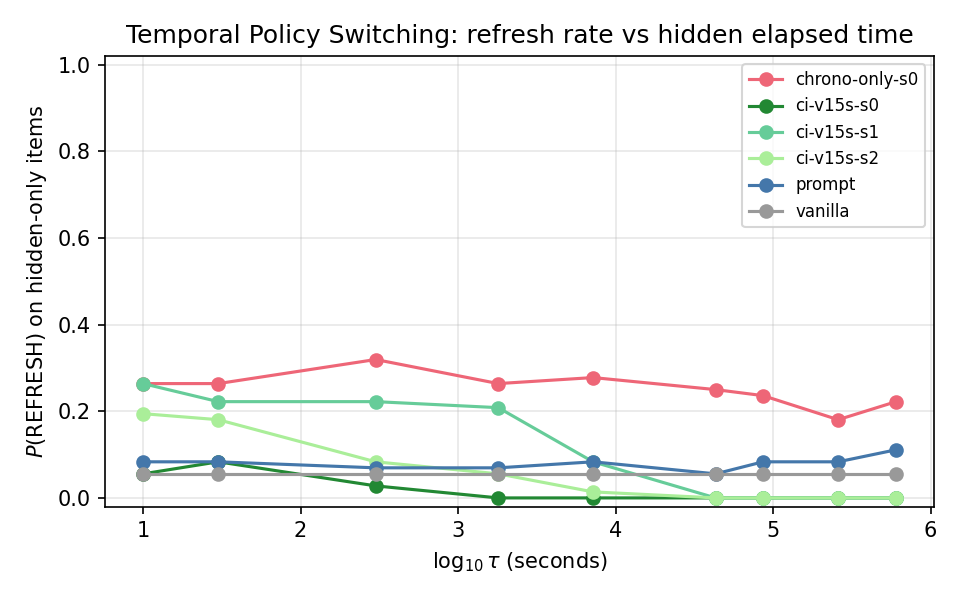
\includegraphics[width=0.95\columnwidth]{figures/fig_tps_monotonicity.png}
\caption{TPS hidden-only: $P(\text{REFRESH})$ as a function of $\log_{10}\Tau$. Vanilla is flat (no signal). \CI{} v15s shows a slight negative slope (refresh becomes less likely as $\Tau$ grows, opposite of expected). chrono-only is closer to flat. None of the adapters tested produce the expected monotonic increase, so the hidden channel does not transfer zero-shot to this policy axis.}
\label{fig:tps-mono}
\end{figure}

\begin{table}[t]
\centering
\caption{TPS conflict condition (108 \emph{fake conflict} items excluded; $n=540$ per adapter). \emph{Scalar-follow}: $P(\text{action matches hidden gold})$. \emph{Prompt-follow}: $P(\text{action matches visible gold})$. \CI{} v15s scalar-follow does not exceed vanilla's, so H3 is inconclusive.}
\label{tab:tps-conflict}
\footnotesize
\begin{tabular}{lcc}
\toprule
Model & Scalar-follow & Prompt-follow \\
\midrule
Vanilla & 0.354 & 0.530 \\
chrono-only (s0) & 0.363 & 0.430 \\
\CI{} v15s (s0) & 0.394 & 0.496 \\
\CI{} v15s (s1) & 0.344 & 0.361 \\
\CI{} v15s (s2) & 0.320 & 0.298 \\
\bottomrule
\end{tabular}
\end{table}

\textbf{Interpretation.} TPS hidden-only tests whether the residual time channel changes downstream action selection under identical visible text. The cross-seed result is negative: \CI{} v15s does not outperform vanilla, and refresh probability does not rise monotonically with $\Tau$. The chrono-only ablation shows a small positive signal on the held-out family, suggesting that some compositional generalization is possible without the LoRA surface, but the effect size is too small to claim a behavioral contribution. This result is consistent with the mechanistic finding that $\Tau$ becomes linearly recoverable from hidden states without becoming a behavioral feature: the channel is \emph{transmitted} but not, in the zero-shot setting tested here, \emph{used} by the model's output policy. We report this negative result because it is the most honest statement of the limits of zero-shot transfer for \CI{}.

\textbf{What this rules out.} TPS rules out the claim that \CI{}, as trained on CLOCK + SILENT-GAP + PHASE, yields a behavior-shaping policy channel that generalizes zero-shot to cache/session/freshness decisions. It does \emph{not} rule out the mechanistic transmission result (Sec.~VI-A), the causal interventions (Sec.~VI-B), or the response-shape result on TPDR (Sec.~VI-F), all of which remain intact.

\textbf{Policy-trained Track B.} To separate zero-shot transfer from task-specific downstream use, we also trained a distinct Track B family on TPS forced-choice policy labels. Track B uses separate training data, checkpoints, reports, and run directories from the Track A mechanistic \CI{} models; the current artifact is \texttt{runs/ci\_track\_b\_policy\_full\_safe\_20260531/reports/track\_b/headline.json}. This is not a replacement for the zero-shot result above. It asks a narrower question: once policy supervision is provided, can the hidden elapsed-time scalar drive action selection under identical visible prompts?

\begin{table}[t]
\centering
\caption{Policy-trained Track B TPS results. \CI{} policy values are cross-seed mean $\pm$ sample standard deviation over seeds 0--2. \emph{Scalar-follow} is measured on prompt/scalar conflict items. $r$ is Spearman correlation between $\log\Tau$ and the probability of the long-delay action on hidden-only items.}
\label{tab:tps-track-b}
\footnotesize
\begin{tabular}{lccccc}
\toprule
Model & Overall & Hidden-only & H/O templ. & H/O fam. & Scalar-follow / $r$ \\
\midrule
Vanilla policy & 0.401 & 0.418 & 0.366 & 0.181 & 0.377 / -0.000 \\
LoRA-only policy (s0) & 0.581 & 0.574 & 0.574 & 0.155 & 0.585 / 0.000 \\
chrono-only policy (s0) & 0.690 & 0.796 & 0.639 & 0.384 & 0.765 / 0.635 \\
\CI{} policy & $0.756\pm0.023$ & $0.871\pm0.030$ & $0.713\pm0.020$ & $0.391\pm0.084$ & $0.871\pm0.029$ / $0.691\pm0.027$ \\
\bottomrule
\end{tabular}
\end{table}

The Track B result supports a policy-trained behavioral claim: with direct TPS supervision, the hidden elapsed-time channel can control forced-choice action selection, follows the hidden scalar under prompt/scalar conflict, and becomes monotone in the intended direction. The caveat is equally important. Held-out-family transfer to \texttt{market\_data} remains weak for policy-trained \CI{} ($0.391\pm0.084$), so this experiment does not establish broad domain generalization. It shows task-specific downstream use of the hidden channel, not that the Track A model already learned a general freshness policy.

\textbf{Limitations.} TPS uses templated synthetic prompts and rule-based oracle labels; a natural-language production benchmark remains open. The conflict numbers in Table~\ref{tab:tps-conflict} exclude 108 fake-conflict items in \texttt{market\_data} where the family threshold equalled the short-side prompt $\Tau$. Several reviewer-requested baselines (prompt-text + LoRA, soft-prompt / prefix tuning, matched-parameter scalar embedding, and larger matched adapters) are deferred to future work. The Track B policy-trained run is separate from the Track A mechanistic run and remains synthetic; its weak held-out-family transfer is the main reason not to claim broad TPS generalization.
